% $Id: template.tex 11 2007-04-03 22:25:53Z jpeltier $

\documentclass{vgtc}
% final (conference style)
%\documentclass[review]{vgtc}                 % review
%\documentclass[widereview]{vgtc}             % wide-spaced review
%\documentclass[preprint]{vgtc}               % preprint
%\documentclass[electronic]{vgtc}             % electronic version

%% Uncomment one of the lines above depending on where your paper is
%% in the conference process. ``review'' and ``widereview'' are for review
%% submission, ``preprint'' is for pre-publication, and the final version
%% doesn't use a specific qualifier. Further, ``electronic'' includes
%% hyperreferences for more convenient online viewing.

%% Please use one of the ``review'' options in combination with the
%% assigned online id (see below) ONLY if your paper uses a double blind
%% review process. Some conferences, like IEEE Vis and InfoVis, have NOT
%% in the past.

%% Figures should be in CMYK or Grey scale format, otherwise, colour 
%% shifting may occur during the printing process.

%% These few lines make a distinction between latex and pdflatex calls and they
%% bring in essential packages for graphics and font handling.
%% Note that due to the \DeclareGraphicsExtensions{} call it is no longer necessary
%% to provide the the path and extension of a graphics file:
%% \includegraphics{diamondrule} is completely sufficient.
%%
\ifpdf%                                % if we use pdflatex
  \pdfoutput=1\relax                   % create PDFs from pdfLaTeX
  \pdfcompresslevel=9                  % PDF Compression
  \pdfoptionpdfminorversion=7          % create PDF 1.7
  \ExecuteOptions{pdftex}
  \usepackage{graphicx}                % allow us to embed graphics files
  \DeclareGraphicsExtensions{.pdf,.png,.jpg,.jpeg} % for pdflatex we expect .pdf, .png, or .jpg files
  \DeclareUnicodeCharacter{FB01}{fi}  % ADDED THIS LINE TO AVOID LIGATURE [MAURO]
\else%                                 % else we use pure latex
  \ExecuteOptions{dvips}
  \usepackage{graphicx}                % allow us to embed graphics files
  \DeclareGraphicsExtensions{.eps}     % for pure latex we expect eps files
\fi%

%% it is recomended to use ``\autoref{sec:bla}'' instead of ``Fig.~\ref{sec:bla}''
\graphicspath{{figures/}{pictures/}{images/}{./}} % where to search for the images

\usepackage{microtype}                 % use micro-typography (slightly more compact, better to read)
\PassOptionsToPackage{warn}{textcomp}  % to address font issues with \textrightarrow
\usepackage{textcomp}                  % use better special symbols
\usepackage{amsmath}                  % use matching math font
\usepackage{times}                     % we use Times as the main font
\renewcommand*\ttdefault{txtt}         % a nicer typewriter font
\usepackage{cite}                      % needed to automatically sort the references
\usepackage{tabu}                      % only used for the table example
\usepackage{booktabs}                  % only used for the table example

%% We encourage the use of mathptmx for consistent usage of times font
%% throughout the proceedings. However, if you encounter conflicts
%% with other math-related packages, you may want to disable it.


%% If you are submitting a paper to a conference for review with a double
%% blind reviewing process, please replace the value ``0'' below with your
%% OnlineID. Otherwise, you may safely leave it at ``0''.
\onlineid{0}

%% declare the category of your paper, only shown in review mode
\vgtccategory{Research}

%% allow for this line if you want the electronic option to work properly
\vgtcinsertpkg

%% In preprint mode you may define your own headline.
%\preprinttext{To appear in an IEEE VGTC sponsored conference.}

%% Paper title.

\title{Drumming in VR - A Case Study}

%% This is how authors are specified in the conference style

%% Author and Affiliation (single author).
%%\author{Roy G. Biv\thanks{e-mail: roy.g.biv@aol.com}}
%%\affiliation{\scriptsize Allied Widgets Research}

%% Author and Affiliation (multiple authors with single affiliations).
%%\author{Roy G. Biv\thanks{e-mail: roy.g.biv@aol.com} %
%%\and Ed Grimley\thanks{e-mail:ed.grimley@aol.com} %
%%\and Martha Stewart\thanks{e-mail:martha.stewart@marthastewart.com}}
%%\affiliation{\scriptsize Martha Stewart Enterprises \\ Microsoft Research}

%% Author and Affiliation (multiple authors with multiple affiliations)
\author{Anca-Simona Horvath\thanks{e-mail: ancah@hum.aau.dk}\\ %
        \scriptsize Humanities, AAU %
\and Mauro Nascimben \thanks{e-mail: mana@create.aau.dk}\\ %
     \scriptsize Augmented Cognition Lab \\ CREATE, AAU CPH %
\and Silvin Willemsen\thanks{e-mail: sil@create.aau.dk}\\ %
     \parbox{1.4in}{\scriptsize \centering Multisensory Experience Lab \\ CREATE, AAU CPH}}

%% A teaser figure can be included as follows, but is not recommended since
%% the space is now taken up by a full width abstract.
%\teaser{
%  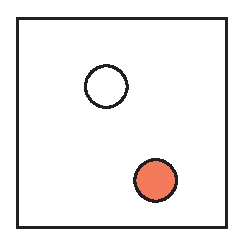
\includegraphics[width=1.5in]{sample.eps}
%  \caption{Lookit! Lookit!}
%}

%% Abstract section.
\abstract{Duis autem vel eum iriure dolor in hendrerit in vulputate
velit esse molestie consequat, vel illum dolore eu feugiat nulla
facilisis at vero eros et accumsan et iusto odio dignissim qui blandit
praesent luptatum zzril delenit augue duis dolore te feugait nulla
facilisi. Lorem ipsum dolor sit amet, consectetuer adipiscing elit,
sed diam nonummy nibh euismod tincidunt ut laoreet dolore magna
aliquam erat volutpat. Ut wisi enim ad minim veniam, quis nostrud exerci tation ullamcorper
suscipit lobortis nisl ut aliquip ex ea commodo consequat. Duis autem
vel eum iriure dolor in hendrerit in vulputate velit esse molestie
consequat, vel illum dolore eu feugiat nulla facilisis at vero eros et
accumsan et iusto odio dignissim qui blandit praesent luptatum zzril
delenit augue duis dolore te feugait nulla facilisi.%
} % end of abstract

%% ACM Computing Classification System (CCS). 
%% See <http://www.acm.org/about/class> for details.
%% We recommend the 2012 system <http://www.acm.org/about/class/class/2012>
%% For the 2012 system use the ``\CCScatTwelve'' which command takes four arguments.
%% The 1998 system <http://www.acm.org/about/class/class/2012> is still possible
%% For the 1998 system use the ``\CCScat'' which command takes four arguments.
%% In both cases the last two arguments (1998) or last three (2012) can be empty.

\CCScatlist{
  \CCScatTwelve{Human-centered computing}{Visu\-al\-iza\-tion}{Visu\-al\-iza\-tion techniques}{Treemaps};
  \CCScatTwelve{Human-centered computing}{Visu\-al\-iza\-tion}{Visualization design and evaluation methods}{}
}

%\CCScatlist{
  %\CCScat{H.5.2}{User Interfaces}{User Interfaces}{Graphical user interfaces (GUI)}{};
  %\CCScat{H.5.m}{Information Interfaces and Presentation}{Miscellaneous}{}{}
%}

%% Copyright space is enabled by default as required by guidelines.
%% It is disabled by the 'review' option or via the following command:
% \nocopyrightspace

%%%%%%%%%%%%%%%%%%%%%%%%%%%%%%%%%%%%%%%%%%%%%%%%%%%%%%%%%%%%%%%%
%%%%%%%%%%%%%%%%%%%%%% START OF THE PAPER %%%%%%%%%%%%%%%%%%%%%%
%%%%%%%%%%%%%%%%%%%%%%%%%%%%%%%%%%%%%%%%%%%%%%%%%%%%%%%%%%%%%%%%%

\begin{document}

%% The ``\maketitle'' command must be the first command after the
%% ``\begin{document}'' command. It prepares and prints the title block.

%% the only exception to this rule is the \firstsection command
\firstsection{Introduction}

\maketitle

In \autoref{sec:sys}, an overview of the complete system will be given. In \autoref{sec:PM} details about the physical model will be 

\section{System Overview} \label{sec:sys}
\textit{NOTES:}
\begin{itemize}
    \item Oculus for VR experience
    \item Leap motion for control
    \item Physical drum for interaction
    \item Haptuator for haptic feedback
    \item Physical model for sound and haptuator input
\end{itemize}

\section{Physical Model}\label{sec:PM}
The behaviour of musical instruments can be well described by partial differential equations (PDEs) \cite{Fletcher1998}. In this section, the continuous-time PDE for a drum-membrane will be given and explained. This is followed by an explanation of the discretisation method after which and parameter values for our implementation will be given. 

\subsection{Continuous time}
A rectangular (stiff) membrane with dimensions $L_x$ (m) and $L_y$ (m) can be described by the following equation \cite{bilbao2009numerical}:

\begin{equation}
\rho H\frac{\partial^2u}{\partial t^2} = T\Delta u - D\Delta\Delta u - 2 \sigma_0\frac{\partial u}{\partial t} + 2 \sigma_1 \Delta \frac{\partial u}{\partial t}.
\end{equation}
Here state variable, $u = u(x,y,t)$ is a function of horizontal coordinate $x \in [0, L_x]$, vertical coordinate $y \in [0, L_y]$ and time $t\geq0$ and is parameterised in terms of material density $\rho$ (kg/m$^3$), membrane thickness $H$ (m), tension $T$ (N) and frequency independent and dependent damping coefficients $\sigma_0$ (s$^{-1}$) and $\sigma_1$ (m$^2$/s). Furthermore, $D = EH^3/12(1-\nu^2)$ with Young's modulus $E$ (Pa) and Poisson's ratio $\nu$. Lastly, $\Delta$ represents the 2D Laplacian \cite{bilbao2009numerical}:
\begin{equation}\label{eq:PDE}
    \Delta = \frac{\partial^2}{\partial x^2} + \frac{\partial^2}{\partial y^2}
\end{equation}

\subsection{Discretisation}
For implementation of the physical model, finite-difference time-domain (FDTD) methods have been used for their accuracy. This technique discretised $u(x,y,t)$ shown in \autoref{eq:PDE} to $u_{(l,m)}^n$ using $x=lh$ where $l \in [0, ..., N_x-1]$ and $y=mh$ where $m \in [0, ..., N_y-1]$ where $N_x$ and $N_y$ are the number of horizontal and vertical grid points respectively. Furthermore, time is discretised using $t = nk$ with sample $n$ and time step $k$ (s) and $h$ (m) is the space between two grid points calculated using 

\begin{equation}\label{eq:h}
    h \geq h_\text{min} =  2\sqrt{\frac{c^2k^2 + 4\sigma_1k + \sqrt{(c^2k^2 + 4\sigma_1k)^2 + 4\kappa^2 k^2} }{2}},
\end{equation}
where $c = \sqrt{T/\rho H}$ and $\kappa = \sqrt{D/\rho H}$. The closer $h$ is to $h_\text{min}$, the higher the accuracy of the implementation. Furthermore, clamped boundary conditions -- i.e., the state $u$ at all plate edges and their gradients are 0 -- have been chosen:
\begin{equation}
    u = \nabla u = 0.
\end{equation}
\\
\subsection{Parameters}
Most parameters used in the simulation were chosen using trial and error and educated guesses \textbf{$\leftarrow$ Probably write something different here :)}. They can be found in \autoref{tab:parameters}.
\begin{table}[h]
\caption{Table showing parameter values}\label{tab:parameters}
\centering
\begin{tabular}{|c|c|c|}
    \hline
    Parameter & Symbol (unit) & Value \\
    \hline
    Membrane width & $L_x$ (m) & $0.3$\\
    Membrane length & $L_y$ (m) & $0.3$ \\
    Material density & $\rho$ (kg/m$^3$)& $10$ \\
    Thickness & $H$ (m) & $0.001$ \\
    Tension & $T$ (N) & $T \in [5, 80]$ \\
    Young's modulus & $E$ (Pa)& $2\cdot 10^3$ \\
    Poisson's ratio & $\nu$ (-)& $0.3$ \\
    Freq. indep. damping & $\sigma_0$ (s$^{-1}$) & $\sigma_0 \in [0, 5]$\\
    Freq. dep. damping & $\sigma_1$ (m$^2$/s) & $\sigma_1 \in [0, 0.005]$\\
    Time step & $k$ (s) & $1/44100$\\
    Grid spacing & $h$ (m) & $4h_\text{min}$\\
    \hline
\end{tabular}
\end{table}\vspace{1em}

\textit{NOTES}
\begin{itemize}
    \item Clamped boundary conditions
    \item Discretisation
    \item Parameter design
\end{itemize}

For speed purposes we multiply $h$ in \autoref{eq:h} by 4.

\section{Haptics}
\subsection{Introduction}
Touch is the first sense to develop in the womb in humans \cite{Barnett1972} compared to visions that it is the last one we develop. Another difference between touch and vision, is that we cannot shut down touch whereas we can close our eyes voluntarily. However tactile awareness always receives less attention than other sensory modalities. One reason for this under-evaluation of tactile stimuli could be the broad number of sensations touch comprises: pressure, temperature, pleasure, pain, joint position, muscle sense, and movement. Probably pain should be included too. 

\subsection{Haptic perception}
Peripheral Nervous System gathers environmental stimuli in form of visual, audible, tactile, olfactive and gustatory inputs and transfers them to the Central Nervous System for further elaboration and integration. Tactile information is collected by proprioceptors in the skin, muscles, and joints and sent to the primary somatosensory cortex (post-central gyrus) via the dorsal column-medial lemniscus pathway to the thalamic nuclei \cite{Blatow2007}. This cortical area is the first stage for the tactile awareness occurring across body surface. The primary somatosensory cortex represents tactile stimuli following an inverted order from the toe (at the top of the parietal hemisphere) to mouth (at the lateral side of the parietal hemisphere) \cite{Narici1999}. However, several other structures of the central nervous system concur in the generation of tactile feedback: generally, a single brain area is never responsible for the awareness of information \cite{Manzoni1986}. Directly connected with the primary somatosensory cortex is the secondary somatosensory cortex, an associative area important in humans for light touch and tactile attention \cite{Eickhoff2005}. It is reported in literature that persons undergoing tactile training improve their perception but also strengthens the connections and cortical representations of the stimulated body area \cite{Saito2007} with a direct relationship between size of cortical region and haptic performance. For the awareness of touch it is also important the presence of short term memory system \cite{Edelman1989}: the parietal ventral area connects both pre-motor brain areas and the somatosensory memory hub. A specific area of the central parietal lobe, placed caudally from the primary somatosensory cortex, integrates the information from the visual and haptic regions to locate objects in space. 

\subsection{Technical notes on experiments involving haptics}
Conducting experiments on haptics it is quite difficult because there aren’t proper technological devices for delivering controlled and reliable tactile stimuli. In Virtual Environments using Leap Motion technology, subjects move freely their hands and this could confound somatosensory processing with activations related to motor planning and movement \cite{Bodegard2001}. These uncontrolled motor activities also result in uncontrolled somatic stimulation. There is an anatomical explanation of this close somato-motor functional relationship: areas involved in the perception of touch on the hands in the primary somatosensory cortex are located mostly in front of the areas responsible for hand movements \cite{Penfield1950}.
Another problem with haptics is the subjective quantification of the stimuli. Contents of tactile consciousness vary between individuals and a common lexicon to evaluate haptic sensation through surveys still seems far to be conceived \cite{Gallace2010}.

\subsection{Interaction between visual information and tactile feedback}
In famous experiment by \cite{Pavani2000}, authors asked a group of persons to detect the position of vibrotactile stimuli while their upper limbs were placed out of view and a fake rubber hand was placed in front of them. Rubber hand was placed in a position that was anatomically-compatible with their real limbs and participants always reported that tactile stimulation was arising from the mannequin and not from their real hand. A similar experiment was conducted by \cite{Schaefer2006} asking subjects to watch a video of a hand being touched on the first finger while their own hand was stimulated synchronously. Brain activity during synchronous stimulation showed an improved tactile acuity.  In Virtual Environments hand manipulations and interactions are a component that enhances realism. 

\section{Myo Armband}
Myo (Thalmic Labs, now North) is a wireless sensor that records surface electromyographic (i.e. sEMG) activity from 8 sensors placed around the forearm. Sensors record EMG signals converting muscle activation in electric potentials. The sampling frequency of the device is 200Hz and the signal amplitude is expressed in “units of activation” and not on mV like standard electromyographic recorders. The armband encloses nine axis inertial measurement unit (i.e. IMU) which contains a three axis gyroscope, three axis accelerometer and a three axis magnetometer \cite{myowebsite}. From these measurements of spatial information, wearer’s arm can be tracked both in the orientation and movement. The orientation data indicates the positioning of the armband in terms of the euler angles (i.e. roll, pitch and yaw). The angular velocity of the armband is provided in a vector format and the accelerometer represents the acceleration the Myo armband is undergoing at a given time. It should be considered that the Myo armband is better suited for determining the relative positioning of the arm rather than the absolute position. The Myo armband has been made to work best at the widest part of the forearm, that is, the upper forearm (Fig. \ref{fig:arm1}).
\begin{figure}[h]
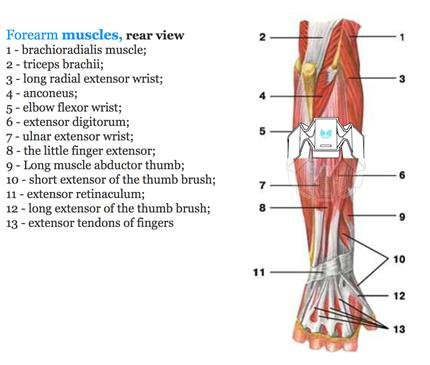
\includegraphics[width=0.5\textwidth]{myo_armband_muscles}
\caption{Muscle detected and armband position}
\centering
\label{fig:arm1}
\end{figure}
Myo can detect the forearm movement in space, flexion and extension of the wirst or when a subject is spreading the fingers or closing the fist. 
\subsection{Raw signals and pre-processing}
To obtain gestural data from a subject after wearing the armband it could be possible to extract the raw signals as shown in Figure \ref{fig:sig0}. The armband uses a bluetooth connection to stream data to the pc for data collection and interpretation. It is suggested from the producer to “warm-up” the band following the app procedure before starting to collect sEMG signals.
\begin{figure}[h]
\includegraphics[width=0.5\textwidth]{signals0}
\caption{Raw sEMG signals as extracted from Myo armband}
\centering
\label{fig:sig0}
\end{figure}
However, raw signals have limited practical application while the common pre-processing involves rectification and envelope calculation (Figure \ref{fig:sig1}). These signals are more easily interpreted and could be integrated in Unity3D environment for hand gesture control. 
\begin{figure}[h]
\includegraphics[width=0.5\textwidth]{signal1}
\caption{Post-processed sEMG signals}
\centering
\label{fig:sig1}
\end{figure}
In Unity3D the arm-band needs to sit on the subject for at least 2 minutes to be considered “stable”. In Unity a simple controller was create using a thin rectangle with a box on the top to simulate a drum-stick. One end-point is fixed in the same way human forearm connects with the arm. The box changes color according to wrist movement in extension (green) or flexion (blue). In other positions the box stays with the gray color. In Figure \ref{fig:mm1}, the extension of the palm of the hand is detected by the system and the color of the box turned to green. Using forearm motion and wrist extension or flexion it could be possible to create a virtual drum using collisions with virtual drum parts. When collision between the virtual stick controlled with Myo and the drum component is detected a wav file could be played with a pre-sampled musical tone. A simple demo was created using this procedure using a cymbal and a snare-drum.
\begin{figure}[h]
\includegraphics[width=0.5\textwidth]{mauro_myo}
\caption{Human interaction in Unity using Myo armband}
\centering
\label{fig:mm1}
\end{figure}

\section{Drumming in Virtual Reality}
\subsection{Myo armband and Leap Motion}
The Leap Motion is a sensor-based cameras and infrared lights that allows accurately track the hands motion, including fingers. Theoretically, it could be possible to combine the data from both Myo armband and Leap Motion in order to create a 3D virtual simulation in real time of an arm motion, including the arm, forearm, hand and fingers. However, for the purposes of this virtual drum project, visualisation of the own hands only is fair enough and the inclusion of the whole arm doesn't improve the whole simulation. For this reason, we built a virtual environment and applied the Leap Motion sensor as shown in Figure \ref{fig:sl1}.
\begin{figure}[h]
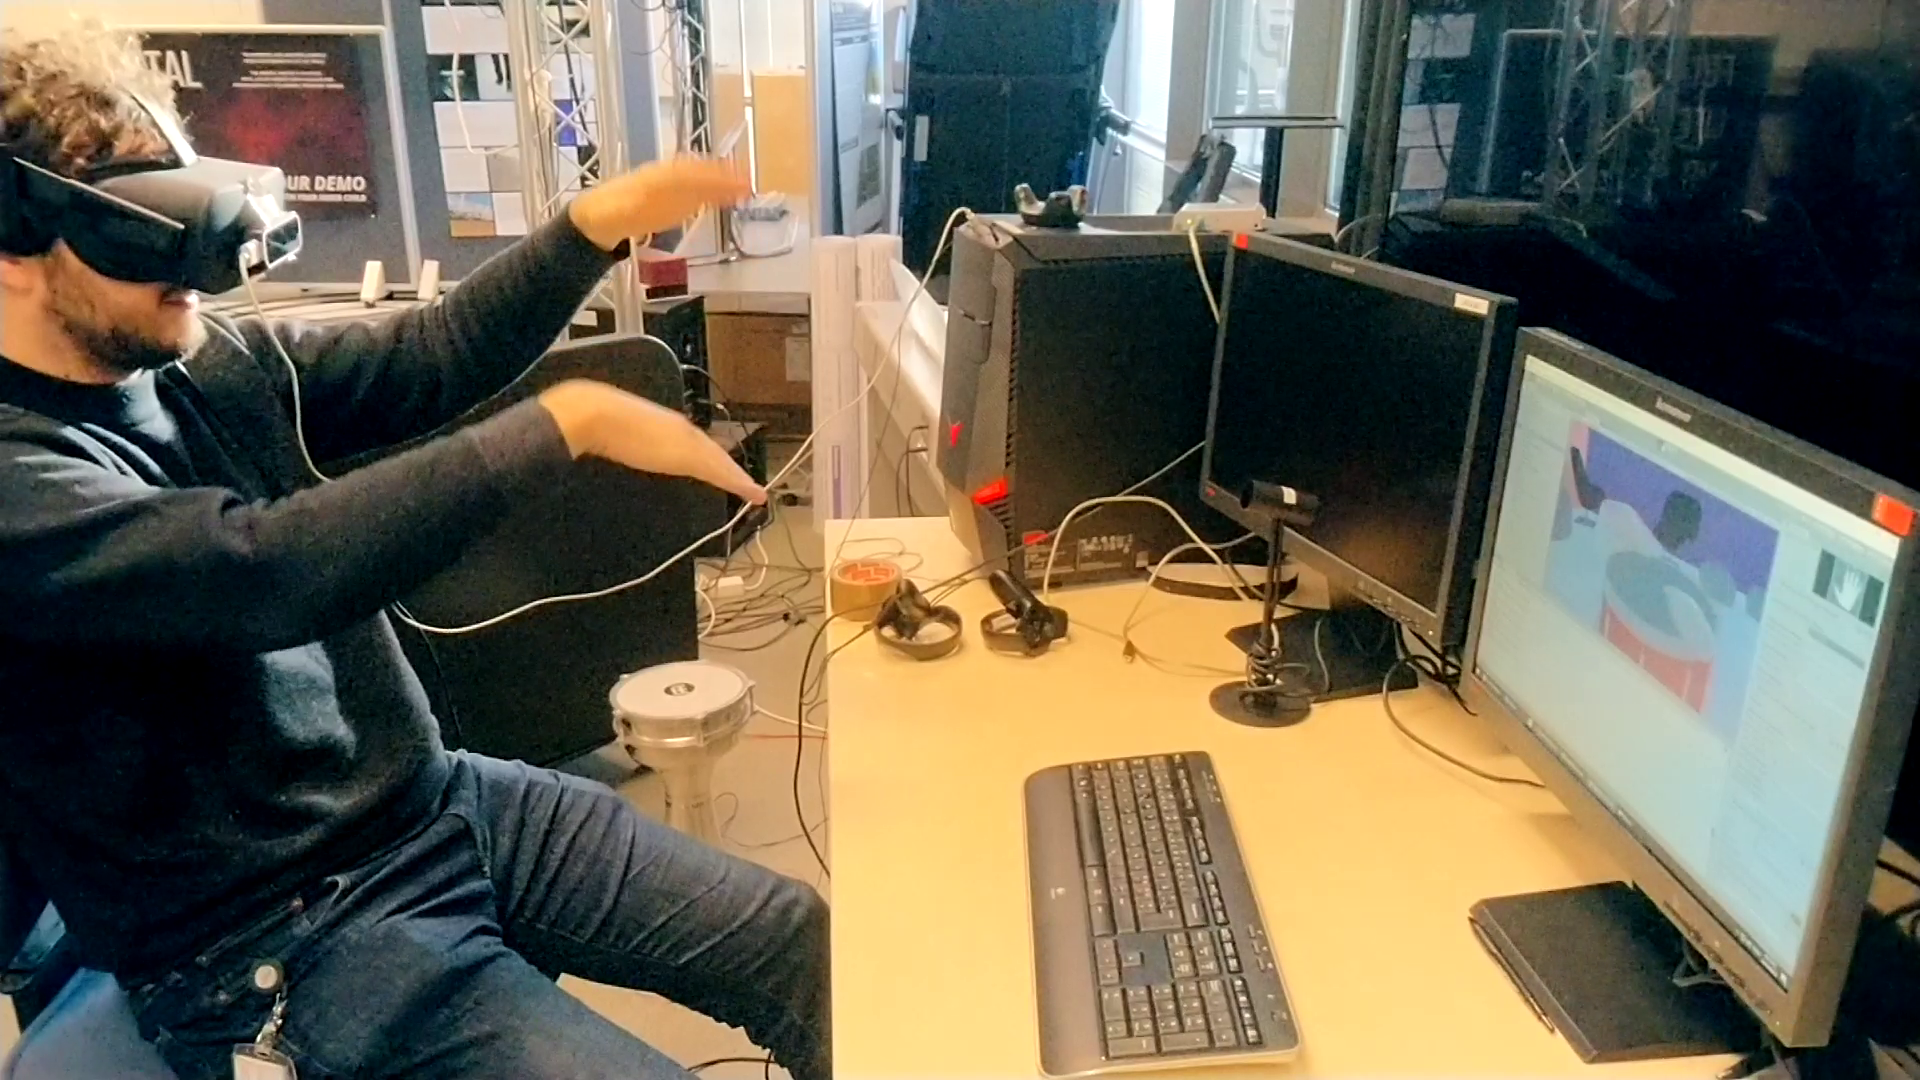
\includegraphics[width=0.5\textwidth]{sil_drum}
\caption{Leap motion and virtual drum}
\centering
\label{fig:sl1}
\end{figure}
\subsection{Virtual Reality environment}
In Unity we created a virtual drum playable with hand motion using Leap Motion sensors. We re-created a virtual room that resembles a recording studio and placed a drum at the center of the room. Drum skin was programmed to detect collision with the reconstructed hand (hand had a capsule collider attached to it). When the collision was detected, the C\# script was activated to reproduce the beating sound of the drum through an actuator placed on the drum skin.
\section{Conclusion}

Lorem ipsum dolor sit amet, consetetur sadipscing elitr, sed diam
nonumy eirmod tempor invidunt ut labore et dolore magna aliquyam erat,
sed diam voluptua. At vero eos et accusam et justo duo dolores et ea
rebum. Stet clita kasd gubergren, no sea takimata sanctus est Lorem
ipsum dolor sit amet. Lorem ipsum dolor sit amet, consetetur
sadipscing elitr, sed diam nonumy eirmod tempor invidunt ut labore et
dolore magna aliquyam erat, sed diam voluptua. At vero eos et accusam
et justo duo dolores et ea rebum. Stet clita kasd gubergren, no sea
takimata sanctus est Lorem ipsum dolor sit amet. Lorem ipsum dolor sit
amet, consetetur sadipscing elitr, sed diam nonumy eirmod tempor
invidunt ut labore et dolore magna aliquyam erat, sed diam
voluptua. At vero eos et accusam et justo duo dolores et ea
rebum.


%% if specified like this the section will be committed in review mode
\acknowledgments{
The authors wish to thank A, B, and C. This work was supported in part by
a grant from XYZ.}

%\bibliographystyle{abbrv}
\bibliographystyle{abbrv-doi}
%\bibliographystyle{abbrv-doi-narrow}
%\bibliographystyle{abbrv-doi-hyperref}
%\bibliographystyle{abbrv-doi-hyperref-narrow}

\bibliography{template}
\end{document}
